\section{実験方法}
筆者はまず半導体スズを室温で安定的に作成した。理化学研究所吉川氏の指導のもと作成した。筆者はスズにGe0.1\%、0.5\%、1\%を混ぜ込んだ試料を作成した。


試料は電気炉とアーク炉を用いて溶融し、水クエンチまたは48時間かけて徐冷した。

\subsection{金属から半導体への転移}
α-β相転移の評価には、家庭用冷凍庫と横磁場マグネットを用いた。

\subsubsection{家庭用冷凍庫での相転移の観察}

\subsubsection{抵抗測定による相転移の評価}

\subsection{電流パルスによる加熱と急冷}

\subsubsection{端子付け}

\subsection{顕微光学実験}
IrTe$_2$試料は理化学研究所(理研)の上谷研究員から提供を受けた。厚さ0.2mm、高さ0.7mm、幅1.3mm程度のバルク試料に二つの電圧端子と二つの電流端子を接続し、試料の抵抗を四端子法を用いて測定した。
試料は光学クライオスタット内に格納し、試料の温度をヘリウム冷凍機とヒーターを用いて制御した。
\begin{figure}[htb]
  \begin{center}
   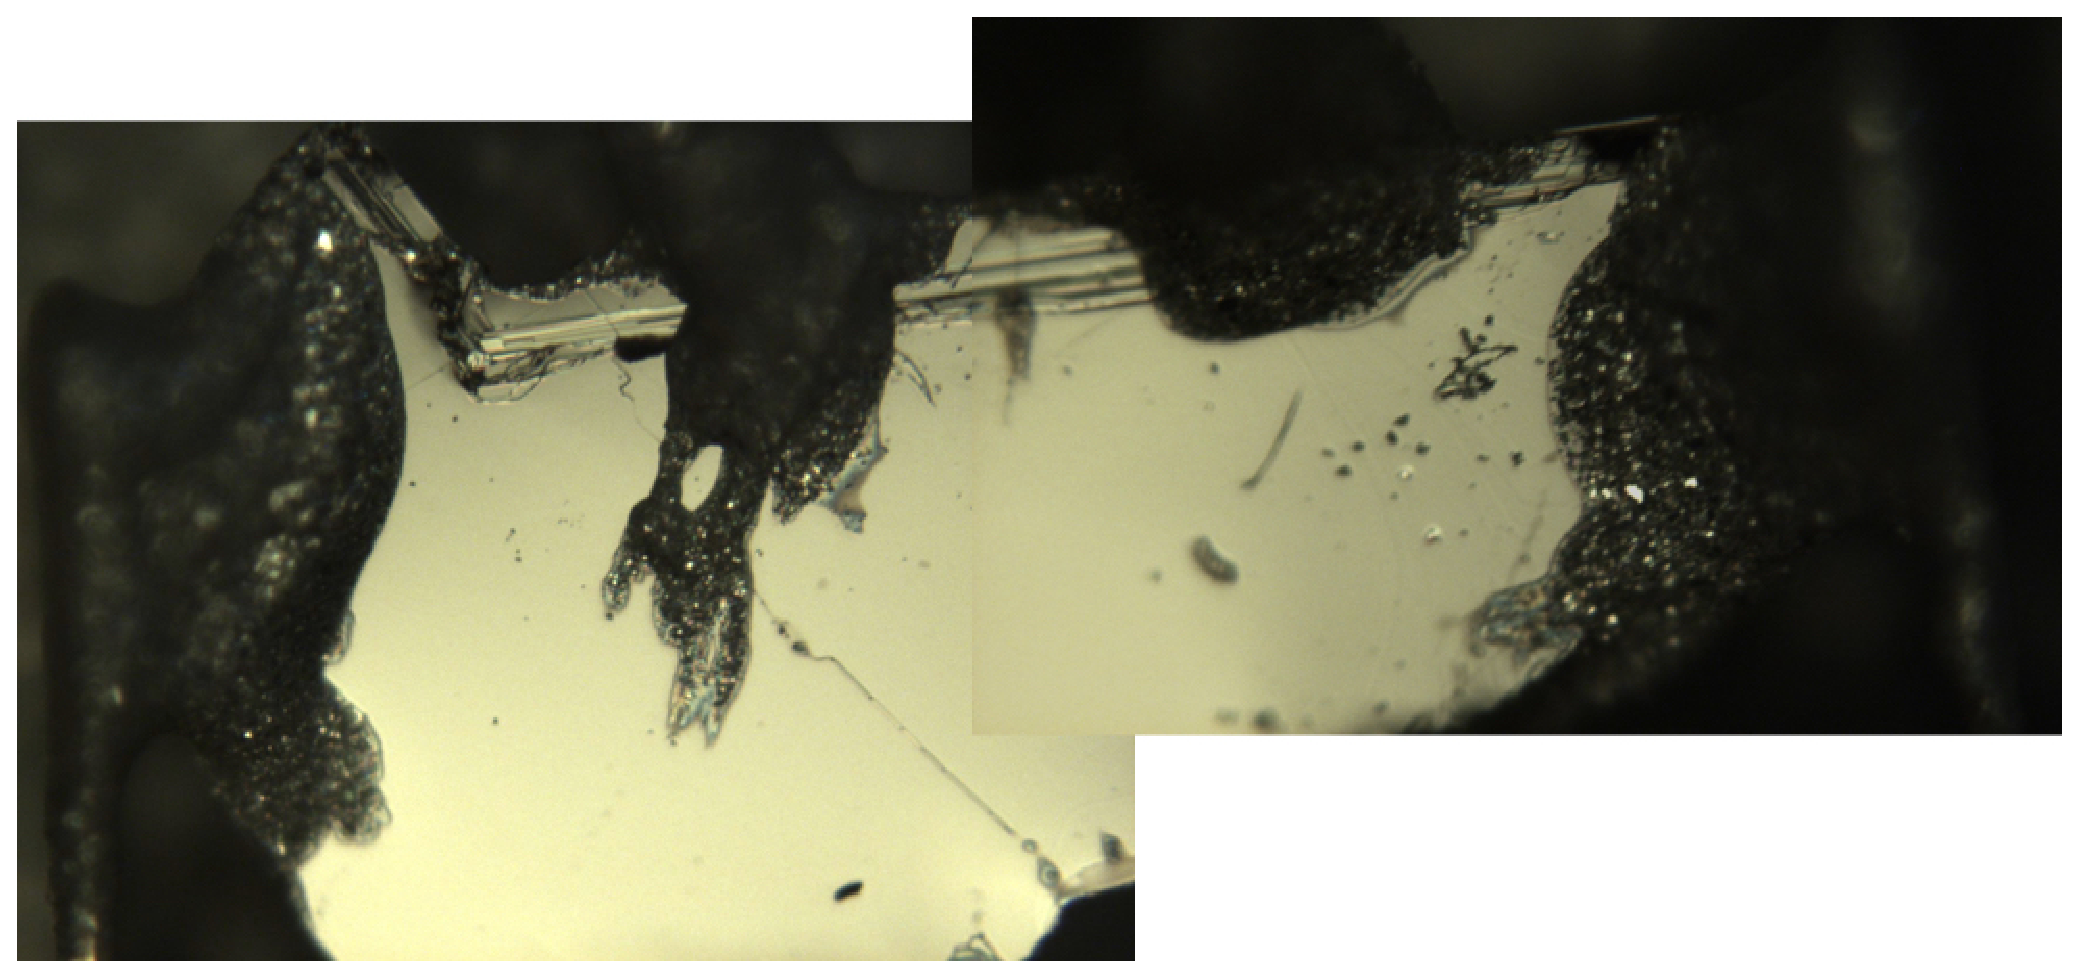
\includegraphics[width=100mm]{experiment/sample.eps}
  \end{center}
  \caption{試料の外観}
  \label{fig:sample}
\end{figure}

\subsubsection{四端子法}
試料に四端子を接続する時の注意点を\ref{sec:4terminal}に書き記す。 四端子を取り付けた後の試料の外観を図\ref{fig:sample}に示した。なお抵抗測定の際にロックインアンプを用いることで信号のSN比を高めた。ロックインアンプの周波数は77Hz、積分時間は1秒にとった。

\subsubsection{偏光顕微光学系}
試料表面の構造を観察するために、反射配置の偏光顕微鏡を構築した。光学系の模式図を図\ref{fig:microscope}に示す。光学素子は光源とコリメータを除き、全てXYZステージの上に固定し、位置を調整できるようにした。白熱ランプ(Edmund製\#MI-150)の赤外域をフィルタでカットした後、ファイバーを通しコリメータ(Edmund製\#LENS ASP0.15)に導き平行光に直した。さらにその平行光を中心波長532nm、半値全幅3nmのバンドパスフィルタ(Thorlabs製\#FL-532-3)に通し、拡散角度$1^\circ$のホログラフィックディフューザー(Edmund製\#47-991)で拡散した。ここでホログラフィックディフューザーを用いたのは、平行光の空間的なコヒーレンスを小さくして照明光に向いたものにするためである。そして消光比15000程度のガラス偏光フィルター(Edmund製\#43-786)を透過させて入射光の偏光を制御し、無偏光ビームスプリッタ(Thorlabs製\#BSW41-532)と対物レンズ(Mitsutoyo製M Plan Apoシリーズ/倍率x10)を通して試料に入射した。ここでビームスプリッタは透過率と反射率がともに偏光状態に依存せず、波長532nm程度で50\%程度となる素子を選定した。試料からの反射光はビームスプリッタで反射され、検光子を通してCCD上に結像するように調整した。光源の後ろとCCDカメラの前にそれぞれ偏光子と検光子としてグラス偏光フィルタを配置し、独立に回転させることで様々な偏光状態に関する偏光顕微鏡像をとった。
\begin{figure}[htb]
  \begin{center}
   \includegraphics[width=100mm,angle=270]{experiment/microscope.eps}
  \end{center}
  \caption{偏光顕微光学系の模式図}
  \label{fig:microscope}
\end{figure}

